% ------------------------------------------------------------------------------
% TYPO3 Version 10.1 - What's New (German Version)
%
% @license	Creative Commons BY-NC-SA 3.0
% @link		http://typo3.org/download/release-notes/whats-new/
% @language	German
% ------------------------------------------------------------------------------

\section{Änderungen für Entwickler}
\begin{frame}[fragile]
	\frametitle{Änderungen für Entwickler}

	\begin{center}\huge{Kapitel 3:}\end{center}
	\begin{center}\huge{\color{typo3darkgrey}\textbf{Änderungen für Entwickler}}\end{center}

\end{frame}

% ------------------------------------------------------------------------------
% Feature | 89054 | Provide core cache frontends via dependency injection

\begin{frame}[fragile]
	\frametitle{Änderungen für Entwickler}
	\framesubtitle{Cache Dependency Injection (1)}

	% decrease font size for code listing
	\lstset{basicstyle=\tiny\ttfamily}

	\begin{itemize}
		\item Extension-Entwickler wird empfohlen, Caches direkt einzuspeisen, statt den CacheManager zu verwenden.
		\item Dies erfordert einige einfache Änderungen, siehe folgendes Beispiel:

		\item \textbf{Vorher:}

\begin{lstlisting}
class MyClass
{
  /**
   * @var TYPO3\CMS\Core\Cache\Frontend\FrontendInterface
   */
  private $cache;

  public function __construct()
  {
      $cacheManager = GeneralUtility::makeInstance(CacheManager::class);
      $this->cache = $cacheManager->getCache('my_cache');
  }
}
\end{lstlisting}

	\end{itemize}

\end{frame}

% ------------------------------------------------------------------------------
% Feature | 89054 | Provide core cache frontends via dependency injection

\begin{frame}[fragile]
	\frametitle{Änderungen für Entwickler}
	\framesubtitle{Cache Dependency Injection (2)}

	% decrease font size for code listing
	\lstset{basicstyle=\tiny\ttfamily}

	\begin{itemize}
		\item Seit \textbf{TYPO3 v10.1}, sollte diese Klasse folgenderweise aussehen:

\begin{lstlisting}
class MyClass
{
  /**
   * @var TYPO3\CMS\Core\Cache\Frontend\FrontendInterface
   */
  private $cache;

  public function __construct(FrontendInterface $cache)
  {
    $this->cache = $cache;
  }
}
\end{lstlisting}

	\end{itemize}

\end{frame}

% ------------------------------------------------------------------------------
% Feature | 89054 | Provide core cache frontends via dependency injection

\begin{frame}[fragile]
	\frametitle{Änderungen für Entwickler}
	\framesubtitle{Cache Dependency Injection (3)}

	% decrease font size for code listing
	\lstset{basicstyle=\tiny\ttfamily}

	\begin{itemize}
		\item ... und folgende Container-Service-Konfiguration ist erforderlich:

\begin{lstlisting}
services:
  cache.my_cache:
    class: TYPO3\CMS\Core\Cache\Frontend\FrontendInterface
    factory: ['@TYPO3\CMS\Core\Cache\CacheManager', 'getCache']
    arguments: ['my_cache']

  MyClass:
    arguments:
      $cache: '@cache.my_cache'
\end{lstlisting}

	\end{itemize}

\end{frame}

% ------------------------------------------------------------------------------
% Feature | 89066 | Add PHP API for Notifications in backend
%
%\begin{frame}[fragile]
%	\frametitle{Changes for Developers}
%	\framesubtitle{Backend Notifications}
%
%	% decrease font size for code listing
%	\lstset{basicstyle=\smaller\ttfamily}
%
%	\begin{itemize}
%		\item A new PHP API provides a simple way to create JavaScript backend notifications.
%		\item For example:
%
%\begin{lstlisting}
%GeneralUtility::makeInstance(NotificationService::class)
%   ->notice('Notice', 'notice');
%\end{lstlisting}
%
%	\end{itemize}
%
%	\begin{figure}
%		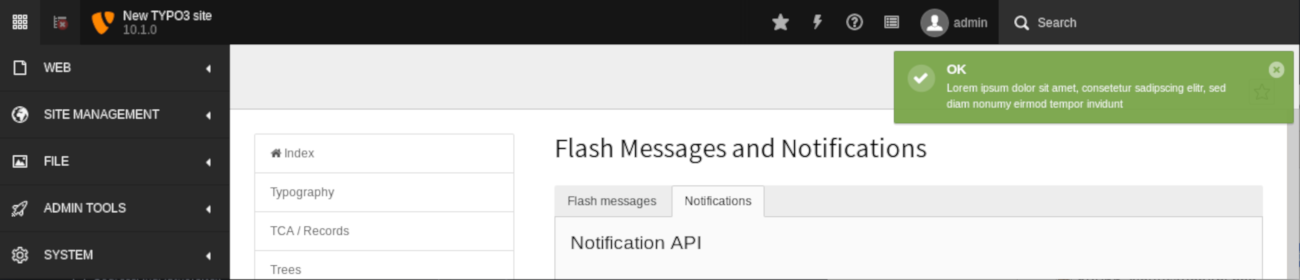
\includegraphics[width=0.90\linewidth]{ChangesForDevelopers/89066-NotificationApi.png}
%	\end{figure}
%
%\end{frame}

% ------------------------------------------------------------------------------
% Feature | 89061 | Introduce Notification Actions

\begin{frame}[fragile]
	\frametitle{Änderungen für Entwickler}
	\framesubtitle{JavaScript Benachrichtigungen}

	\begin{itemize}
		\item JavaScript Benachrichtigungen im BE unterstützen nun Buttons.
	\end{itemize}

	\begin{figure}
		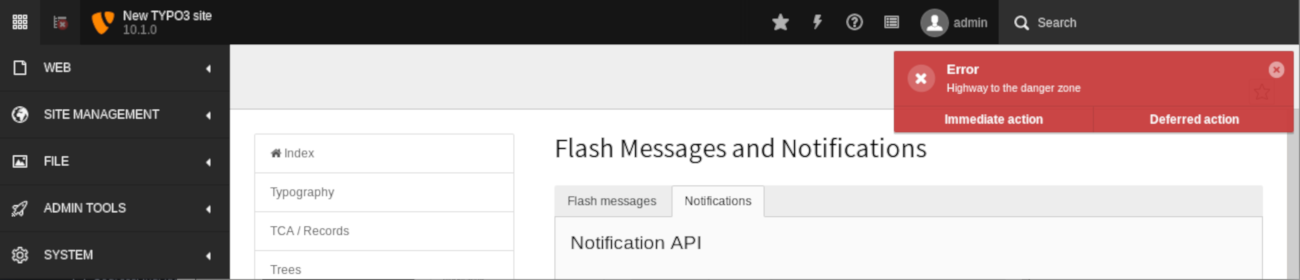
\includegraphics[width=0.90\linewidth]{ChangesForDevelopers/89061-NotificationActionsAndButtons.png}
	\end{figure}

\end{frame}

% ------------------------------------------------------------------------------
% Feature | 89244 | Broadcast Channels and Messaging

\begin{frame}[fragile]
	\frametitle{Änderungen für Entwickler}
	\framesubtitle{Broadcast-Kanäle und Messaging (1)}

	% decrease font size for code listing
	\lstset{basicstyle=\tiny\ttfamily}

	\begin{itemize}
		\item Es ist jetzt möglich, 'Broadcast-Nachrichten' mit JavaScript zu senden und zu empfangen.
	\end{itemize}

	\vspace{-0.2cm}
	\begingroup
		\color{red}
			\begin{center}
				Die API wird vorerst als \textbf{intern} betrachtet\newline
				und kann sich jederzeit ändern, bis sie als 'stabil' betrachtet wird.
			\end{center}
	\endgroup

	\begin{itemize}
		\item Beispiel für das \textbf{Senden} einer Nachricht:

\begin{lstlisting}
require(['TYPO3/CMS/Backend/BroadcastService'], function (BroadcastService) {
  const payload = {
    componentName: 'my_extension',
    eventName: 'my_event',
    foo: 'bar'
  };
  BroadcastService.post(payload);
});
\end{lstlisting}

	\end{itemize}

\end{frame}

% ------------------------------------------------------------------------------
% Feature | 89244 | Broadcast Channels and Messaging

\begin{frame}[fragile]
	\frametitle{Änderungen für Entwickler}
	\framesubtitle{Broadcast-Kanäle und Messaging (2)}

	% decrease font size for code listing
	\lstset{basicstyle=\tiny\ttfamily}

	\begin{itemize}
		\item Beispiel für den \textbf{Empfang} der Nachricht:

\begin{lstlisting}
define([], function() {
  document.addEventListener('typo3:my_component:my_event', (e) => eventHandler(e.detail));
  function eventHandler(detail) {
    // output contains key 'foo' as the payload
    console.log(detail);
  }
});
\end{lstlisting}

		\item Siehe \href{https://developer.mozilla.org/en-US/docs/Web/API/Broadcast_Channel_API}{developer.mozilla.org} für weitere Details.

	\end{itemize}

\end{frame}

% ------------------------------------------------------------------------------
% Feature | 89018 | Provide implementation for PSR-17 HTTP Message Factories

\begin{frame}[fragile]
	\frametitle{Änderungen für Entwickler}
	\framesubtitle{PSR-17 HTTP Message Factories}

	\begin{itemize}
		\item Die \href{https://www.php-fig.org/psr/psr-17/}{PSR-17}
			HTTP Message Factories Implementierung wurde hinzugefügt.
		\item HTTP Message Factory-Schnittstellen sollten als Abhängigkeiten für 
			Anforderungshandler oder Dienste verwendet werden, die PSR-7-Nachrichtenobjekte erstellen.
		\item PSR-17 besteht aus sechs Factory Schnittstellen:

			\begin{itemize}\smaller
				\item \texttt{\textbackslash
					Psr\textbackslash
					Http\textbackslash
					Message\textbackslash
					RequestFactoryInterface}
				\item \texttt{\textbackslash
					Psr\textbackslash
					Http\textbackslash
					Message\textbackslash
					ResponseFactoryInterface}
				\item \texttt{\textbackslash
					Psr\textbackslash
					Http\textbackslash
					Message\textbackslash
					ServerRequestFactoryInterface}
				\item \texttt{\textbackslash
					Psr\textbackslash
					Http\textbackslash
					Message\textbackslash
					StreamFactoryInterface}
				\item \texttt{\textbackslash
					Psr\textbackslash
					Http\textbackslash
					Message\textbackslash
					UploadedFileFactoryInterface}
				\item \texttt{\textbackslash
					Psr\textbackslash
					Http\textbackslash
					Message\textbackslash
					UriFactoryInterface}

			\end{itemize}\normalsize

		\item Siehe die
			\href{https://docs.typo3.org/c/typo3/cms-core/master/en-us/Changelog/10.1/Feature-89018-ProvideImplementationForPSR-17HTTPMessageFactories.html}{Dokumentation}
			für ein Beispiel im Code.

	\end{itemize}

\end{frame}

% ------------------------------------------------------------------------------
% Feature | 89216 | PSR-18 HTTP Client Implementation

\begin{frame}[fragile]
	\frametitle{Änderungen für Entwickler}
	\framesubtitle{PSR-18 HTTP Client}

	\begin{itemize}
		\item Der \href{https://www.php-fig.org/psr/psr-18/}{PSR-18}
			HTTP Client Implementierung wurde hinzugefügt.
		\item Entwickler können HTTP-Anforderungen basierend auf PSR-7 Nachrichtenobjekten generieren
			ohne auf eine bestimmte HTTP-Client-Implementierung angewiesen zu sein.
		\item Dies ersetzt den vorhandenen Wrapper \href{http://guzzlephp.org/}{Guzzle}
			nicht, sondern bietet eine gewöhnlichere Alternative. 
		\item PSR-18 besteht aus einer Client-Schnittstelle und drei Ausnahmeschnittstellen:

			\begin{itemize}\smaller
				\item \texttt{\textbackslash
					Psr\textbackslash
					Http\textbackslash
					Client\textbackslash
					ClientInterface}
				\item \texttt{\textbackslash
					Psr\textbackslash
					Http\textbackslash
					Client\textbackslash
					ClientExceptionInterface}
				\item \texttt{\textbackslash
					Psr\textbackslash
					Http\textbackslash
					Client\textbackslash
					NetworkExceptionInterface}
				\item \texttt{\textbackslash
					Psr\textbackslash
					Http\textbackslash
					Client\textbackslash
					RequestExceptionInterface}
			\end{itemize}\normalsize

		\item Siehe die
			\href{https://docs.typo3.org/c/typo3/cms-core/master/en-us/Changelog/10.1/Feature-89216-PSR-18HTTPClientImplementation.html}{Documentation}
			für ein Codebeispiel.

	\end{itemize}

\end{frame}

% ------------------------------------------------------------------------------
% Feature | 88871 | Handle middleware handler in RequestFactory correctly

\begin{frame}[fragile]
	\frametitle{Änderungen für Entwickler}
	\framesubtitle{RequestFactory Middleware Handler}

	% decrease font size for code listing
	\lstset{basicstyle=\tiny\ttfamily}

	\begin{itemize}
		\item Es ist jetzt möglich, benutzerdefinierte Middleware-Handler als Array zu definieren.
		\item Die RequestFactory erstellt einen Handler-Stack basierend auf dem Array\newline
			\small
				\texttt{\$GLOBALS['TYPO3\_CONF\_VARS']['HTTP']['handler']}
			\normalsize
			und injiziert ihn in den Client.
		\item Zum Beispiel:

\begin{lstlisting}
use \TYPO3\CMS\Core\Utility\GeneralUtility;
use \Vendor\MyExtension\Middleware\Guzzle\CustomMiddleware;
use \Vendor\MyExtension\Middleware\Guzzle\SecondCustomMiddleware;

# Add custom middleware to default Guzzle handler stack
$GLOBALS['TYPO3_CONF_VARS']['HTTP']['handler'][] =
  (GeneralUtility::makeInstance(CustomMiddleware::class))->handler();
$GLOBALS['TYPO3_CONF_VARS']['HTTP']['handler'][] =
  (GeneralUtility::makeInstance(SecondCustomMiddleware::class))->handler();
\end{lstlisting}

	\end{itemize}

\end{frame}

% ------------------------------------------------------------------------------
% Feature | 88602 | Allow registering additional file processors

\begin{frame}[fragile]
	\frametitle{Änderungen für Entwickler}
	\framesubtitle{Benutzerdefinierte Dateiprozessoren}

	% decrease font size for code listing
	\lstset{basicstyle=\tiny\ttfamily}

	\begin{itemize}
		\item Entwickler können nun ihre eigenen Dateiprozessoren registrieren.
		\item Fügen Sie diesen Code in die Datei \texttt{ext\_localconf.php} ein:

\begin{lstlisting}
$GLOBALS['TYPO3_CONF_VARS']['SYS']['fal']['processors']['ExampleImageProcessor'] = [
  'className' => \Vendor\MyExtension\Resource\Processing\ExampleImageProcessor::class,
  'before' => 'LocalImageProcessor',
];
\end{lstlisting}

		\item Typische Anwendungsfälle:

			\begin{itemize}
				\item Wasserzeichen auf Bilder setzen
				\item hochgeladene Dateien in ein ZIP-Archiv komprimieren
				\item bearbeitete Kopien von Bildern speichern
				\item usw.
			\end{itemize}

	\end{itemize}

\end{frame}

% ------------------------------------------------------------------------------
% Feature | 88995 | Calling registerPlugin with vendor name

\begin{frame}[fragile]
	\frametitle{Änderungen für Entwickler}
	\framesubtitle{Extbase und Fluid}

	% decrease font size for code listing
	\lstset{basicstyle=\smaller\ttfamily}

	\begin{itemize}
		\item Lassen Sie den Anbieternamen weg, wenn Sie Plugins mit\newline
			\smaller
				\texttt{\textbackslash
					TYPO3\textbackslash
					CMS\textbackslash
					Extbase\textbackslash
					Utility\textbackslash
					ExtensionUtility::registerPlugin()} registrieren.
			\normalsize

		\item Verwenden Sie beispielsweise "\texttt{Form}" stat "\texttt{TYPO3.CMS.Form}"\newline
			\small(erstes Argument)\normalsize

\begin{lstlisting}
\TYPO3\CMS\Extbase\Utility\ExtensionUtility::registerPlugin(
  'Form',
  'Formframework',
  'Form',
  'content-form',
);
\end{lstlisting}

	\end{itemize}

\end{frame}

% ------------------------------------------------------------------------------
% Important | 89001 | TSFE->createHashBase
% Feature | 89150 | Add events before and after rollback of record history entries

\begin{frame}[fragile]
	\frametitle{Änderungen für Entwickler}
	\framesubtitle{Sonstiges (1)}

	\begin{itemize}
		\item Die \texttt{hashParameters} zur Berechnung der HashBase in der folgenden Klasse wurden geändert:\newline
			\small
				\texttt{TYPO3\textbackslash
					CMS\textbackslash
					Frontend\textbackslash
					Controller\textbackslash
					TypoScriptFrontendController}
			\normalsize

			\begin{itemize}
				\item \texttt{gr\_list} wurde durch \texttt{groupIds} ersetzt.
				\item \texttt{cHash} wurde durch \texttt{dynamicArguments} ersetzt.
				\item \texttt{domainStartPage} wurde durch \texttt{site} (site identifier) ersetzt.
			\end{itemize}

		\item Zwei neue Ereignisse werden ausgelöst, wenn Datensätze zurückgesetzt werden:

			\begin{itemize}\smaller
				\item \texttt{TYPO3\textbackslash
					CMS\textbackslash
					Backend\textbackslash
					History\textbackslash
					Event\textbackslash
					BeforeHistoryRollbackStartEvent}
				\item \texttt{TYPO3\textbackslash
					CMS\textbackslash
					Backend\textbackslash
					History\textbackslash
					Event\textbackslash
					AfterHistoryRollbackFinishedEvent}
			\end{itemize}\normalsize

	\end{itemize}

\end{frame}

% ------------------------------------------------------------------------------
% Feature | 88805 | Add type to TYPO3/CMS/Core/Database/Query/QueryBuilder::set()

\begin{frame}[fragile]
	\frametitle{Änderungen für Entwickler}
	\framesubtitle{Sonstiges (2)}

	\begin{itemize}
		\item Die Methode \texttt{set()} des Abfrage-Generators akzeptiert jetzt ein viertes Argument,
			um den Typ des benannten Parameters anzugeben:\newline
			\small
				\texttt{TYPO3\textbackslash
					CMS\textbackslash
					Core\textbackslash
					Database\textbackslash
					Query\textbackslash
					QueryBuilder::set()}
			\normalsize\newline
			\vspace{0.2cm}
			(der Standardwert ist \texttt{\textbackslash PDO::PARAM\_STR})

	\end{itemize}

\end{frame}

% ------------------------------------------------------------------------------
